\documentclass[sutton_barto_notes.tex]{subfiles}
\begin{document}


\newpage
\section{Eligibility Traces}

There are two ways to view eligibility traces. The more theoretical view, which we emphasize here, is that they are a bridge from TD to Monte Carlo methods. When TD methods are augmented with eligibility traces they produce a family of methods spanning a spectrum that has Monte Carlo methods at one end and 1-step TD methods on the other. In between are intermediate methods that are often better than either extreme method. In this sense eligibility traces unify TD and Monte Carlo methods in a valuable and revealing way.

The other way to view eligibility traces is more mechanistic. From this perspective, an eligibility trace is a temporary record of the occurrence of an event, such as the visiting of a state or the taking of an action. The trace marks the memory parameters associated with the event as eligible for undergoing learning changes. When a TD error occurs, only the eligible states or actions are assigned credit or blame for the error. Thus, eligibility traces help bridge the gap between events and training information. Like TD methods themselves, eligibility traces are a basic mechanism for temporal credit assignment.

For reasons that will become apparent shortly, the more theoretical view of eligibility traces is called the forward view, and the more mechanistic view is called the backward view. The forward view is most useful for understanding what is computed by methods using eligibility traces, whereas the backward view is more appropriate for developing intuition about the algorithms themselves. 

\newpage
\begin{itemize}
\item Eligibility Traces (ET) is a basic mechanism of RL (in TD($\lambda$) the $\lambda$ refers to the use of ET) 
\item Almost any TD method (Q-learning, Sarsa), can be combined with ET 
\item It unifies and generalizes TD ($\lambda = 0$) and MC ($\lambda = 1$) methods 
\item ET provides a way to use MC online, or in continuing problems 
\end{itemize}

 Core of the method: 
\begin{itemize}
\item maintain a short term vector $\mathbf{z}_t \in \mathbb{R}^d$ that parallels the long term vector $\mathbf{w}_t$ 
\item when a component of $\mathbf{w}_t$ participates in producing an estimated value, then the corresponding component of $\mathbf{z}_t$ is bumped up and then begins to fade away 
\item if a non-zero TD error occurs before the trace fades away, we have learning (trace-decay $\lambda \in [0, 1]$) 
\end{itemize}

Advantages of ET over $n$-step methods: 
\begin{itemize}
\item computational advantage: stores only one trace $\mathbf{z}$ rather than the result of $n$ steps in the future (storing last $n$ feature vectors)
\item continually and uniformly learning, rather than delayed learning and all-at-once update at the end
\begin{itemize}
	\item learning occurs and affects behavior immediately
\end{itemize}
\item ET is a \textit{backward} view instead of a \textit{forward} view, which is less complex to implement 
\end{itemize}

\subsection{The lambda return (n-step return with FA)}

 We apply the $n$-step return from chapter 7 to function estimation. The n-step return is the first n rewards + the estimated value of the state reached in n steps, each appropriately discounted: 

\begin{align}
G_{t:t+n} = R_{t+1} + \gamma R_{t+2} + ... + \gamma^{n-1} R_{t+n} + \gamma^n \hat{v}_{t+n-1}(S_{t+n}, \mathbf{w}_{t+n-1}) \label{eq:12.1}\tag{12.1}
\end{align}

\begin{itemize}
\item A valid update can be done towards any n-step return, but also towards any \textbf{average} of n-step returns 
\item For example, target could be half the two step return + half the 4 steps return 
\item Any set can be averaged as long as the weights are positive and sum to 1 
\item We could average one-step and infinite-step returns to get a way of interrelating TD and MC methods 
\item \textbf{Compound update}: Update that averages simpler components 
\end{itemize}

 The TD($\lambda$) algorithm can be viewed as a particular way of averaging n-step updates, each weighted by $\lambda{(n-1)}$ and normalized by $(1 - \lambda)$ to ensure the weights sum to 1: 

\begin{figure}[h!]
    \centering
     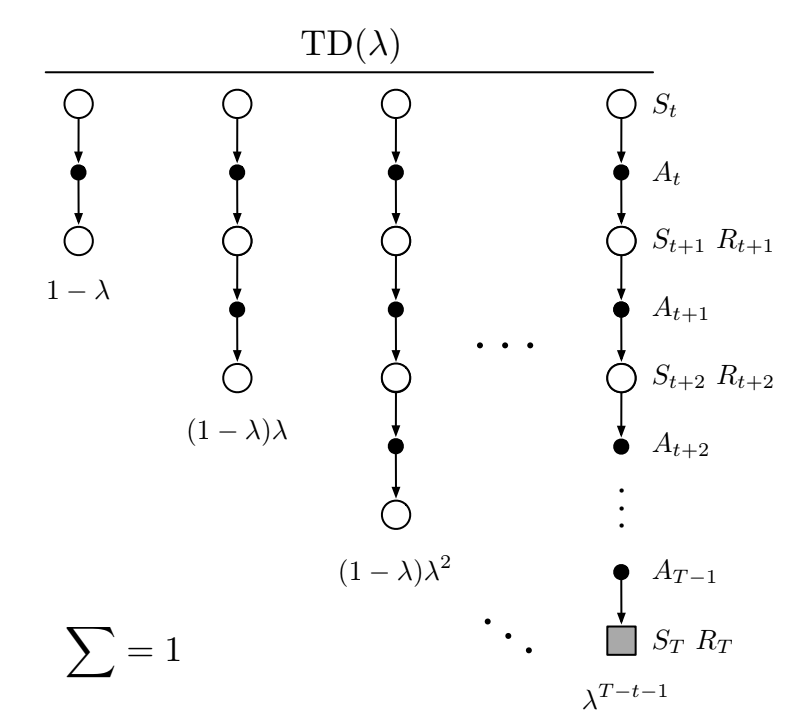
\includegraphics[width=0.6\textwidth]{td_lambda2.png}
    \caption{ Backup diagram for TD($\lambda$). $\lambda = 0$ reduces to the first component only (one-step TD), whereas $\lambda = 1$ gives the full MC update. }
\end{figure}


 The resulting update is towards the \textbf{lambda return}: 

\begin{align}G_t^{\lambda} = (1 - \lambda) \sum_{n=1}^{\infty} \lambda^{n-1} G_{t:t+n} \label{eq:12.2}\tag{12.2}
\end{align}

\newpage
 Weighting illustration: 
\begin{figure}[h!]
    \centering
     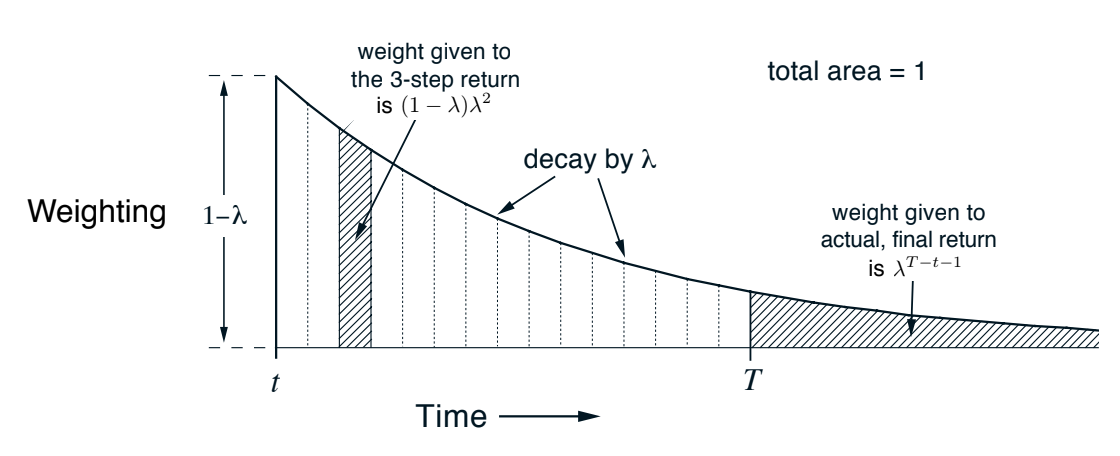
\includegraphics[width=0.8\textwidth]{td_lambda_weights.png}
    \caption{ Weighting for each of the n-step returns in the $\lambda$-return. }
\end{figure}

 First algorithm based on the lambda-return: offline $\lambda$-return algorithm: 
\begin{itemize}
\item offline: waits until the end of the episode to make updates 
\item semi gradient update using the $\lambda$-return as a target 
\end{itemize}
\begin{align}\mathbf{w}_{t+1} = \mathbf{w}_t + \alpha[G_t^{\lambda} - \hat{v}(S_t, \mathbf{w}_t)] \; \nabla \hat{v}(S_t, \mathbf{w}_t), \quad \quad t = 0, ... T-1 \label{eq:12.3}\tag{12.3}\end{align}
\begin{itemize}
\item this is a way of moving smoothly between one-step TD and MC 
\item theoretical, \textbf{forward} view learning algorithm 
\end{itemize}
\begin{figure}[h!]
    \centering
     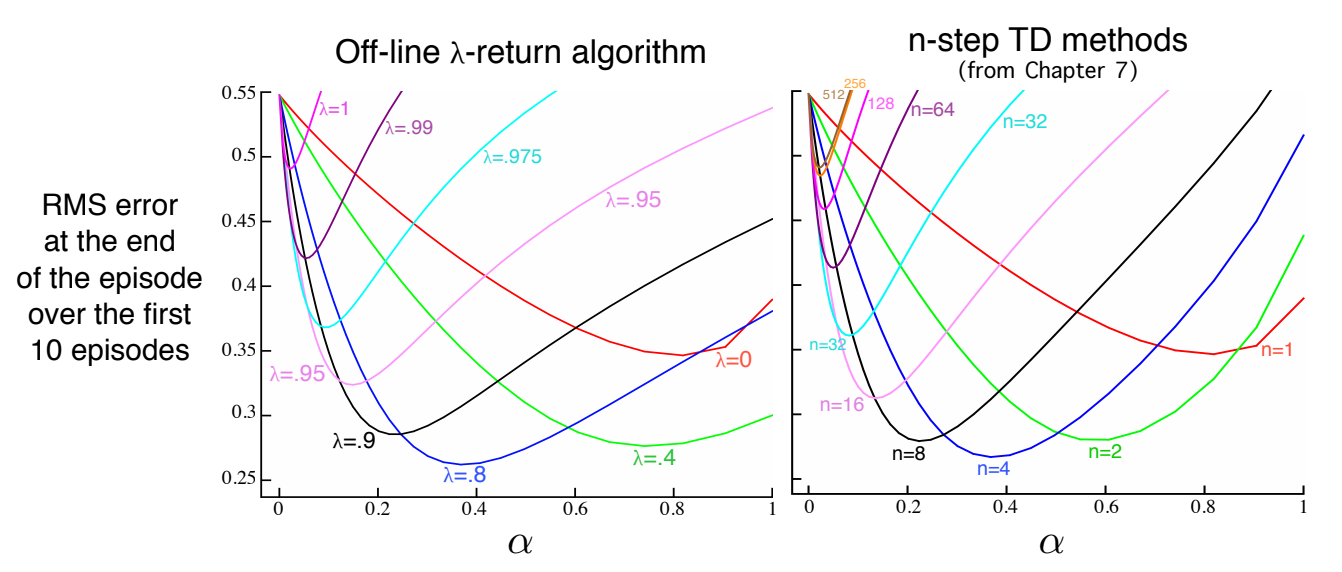
\includegraphics[width=0.8\textwidth]{td_lambda_results.png}
    \caption{ Comparison of $\lambda$-return algorithm vs $n$-step TD methods on a 19 states Random Walk example. $\lambda$-return results are slightly better at the best $\alpha$ and $\lambda$ values, and at high $\alpha$. }
\end{figure}

\newpage
\subsection{TD($\lambda$)}

\begin{itemize}
\item oldest and most widely used RL algorithms 
\item first algorithm with a relation between a theoretical forward view and a more practical backward view. The forward view is the “standard” way like n-step, where the update for a state visited at time $t$ depends on the \textit{future} reward up to $t+n$, which means we have to wait n steps before having enough information to update the “past”. The \textbf{backward} view like ET, maintains the trace vector $\mathbf{z}$ so that the update can be made at the same time. 
\item TD-lambda approximates the off-line $\lambda$-return algorithm of section 12.1, improving it in 3 ways:
    \begin{itemize}
    \item updates the weight vector at every step and not just at the end of the episode 
    \item computations distributed in time rather than at the end 
    \item can be used in continuing problems 
    \end{itemize}
   
\end{itemize}

 In this section we present the semi-gradient version of TD($\lambda$) with function approximation: 
\begin{itemize}
\item the \textbf{eligibility trace} $\mathbf{z}$ has the same dimension as $\mathbf{w}$, initialized to $0$ 
\item it is incremented at each time step by the value gradient 
\item it is decayed at each time step by $\gamma \lambda$ 
\end{itemize}
\begin{align}\mathbf{z}_t = \gamma \lambda \mathbf{z}_{t-1} + \nabla \hat{v}(S_t, \mathbf{w}_t) \quad \quad \quad 0 \leq t \leq T \label{eq:12.4}\tag{12.4}
\end{align}
\begin{itemize}
\item $\gamma$ is the discount rate, $\lambda$ is the trace-decay parameter 
\item \ref{eq:12.4} aka accumulating trace
\end{itemize}

 In linear function approximation, the gradient is just the feature vector $\mathbf{x}_t$ in which case the ET vector is just a sum of past, fading, input vector. 

 The $\mathbf{z}$ components represent the \textbf{“eligibility”} of each component to learning when a reinforcing event occurs. These reinforcing events are moment-by-moment one-step TD errors: 
\begin{align}\delta_t = R_{t+1} + \gamma \hat{v}(S_{t+1}, \mathbf{w}_t) - \hat{v}(S_t, \mathbf{w}_t) \label{eq:12.5}\tag{12.5}\end{align}
 In TD($\lambda$), the weight vector is updated on each step proportional to the scalar TD error and the vector eligibility trace: 
\begin{align}\mathbf{w}_{t+1} = \mathbf{w}_t + \alpha \delta_t \mathbf{z}_t \label{eq:12.6}\tag{12.6}\end{align}

\begin{figure}[h!]
    \centering
     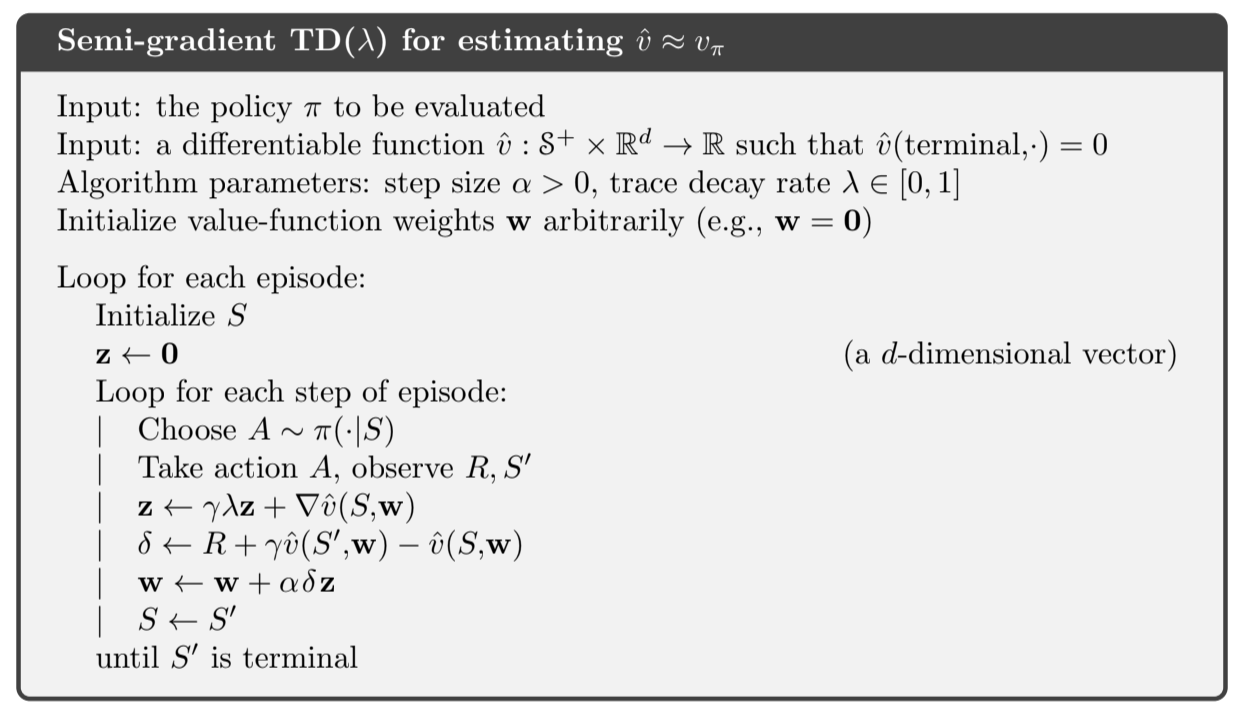
\includegraphics[width=0.8\textwidth]{semigrad_td_lambda.png}
    \caption{ Semi-gradient TD lambda }
\end{figure}

 We have our backward view! At each moment the current TD error is assigned to each prior state according to how much the state contributed to the current ET 
\begin{itemize}
\item TD(1) can be viewed as a more general MC method. $\lambda = 1$ means that all preceding states are given credit like MC but it can be used in an online continuing setting 
\item linear-TD($\lambda$) has been proven to converge in the on-policy case if the step-size parameter is reduced over time (see chap 2.7) 
\item convergence is not to the minimum-error weight vector but to a nearby weight vector that depends on $\lambda$ 
\end{itemize}

\subsection{n-step truncated lambda-return methods}

\begin{itemize}
\item offline $\lambda$-return is limited because we don’t know the $\lambda$-return before the end of the episode 
\item it is problematic in the continuing case because the $\lambda$-return can depend on an arbitrary large n 
\item the dependence falls by $\gamma \lambda$ for each step of delay, so maybe we can just truncate it when it’s small enough 
\item we do this by introducing \textbf{horizon} $h$ which has the same role as time of termination $T$ 
\item in the $\lambda$-return there is a residual weighting given to the true return, here it’s to the longest available n-step return 
\end{itemize}
\begin{align}G_{t:h}^{\lambda} = (1 - \lambda) \sum_{n=1}^{h-t-1} \lambda^{n-1} G_{t:t+n} \quad + \quad \lambda^{h-t-1}G_{t:h} \label{eq:12.7}\tag{12.7}\end{align}
 We use this return in the update: 
\begin{align}\mathbf{w}_{t+n} = \mathbf{w}_{t+n-1} + \alpha [G_{t:t+n}^{\lambda} - \hat{v}(S_t, \mathbf{w}_{t+n-1})] \nabla \hat{v}(S_t, \mathbf{w}_{t+n-1}) \label{eq:12.8}\tag{12.8}\end{align}
 This can be implemented to start updates at $n-1$.
\begin{figure}[h!]
    \centering
     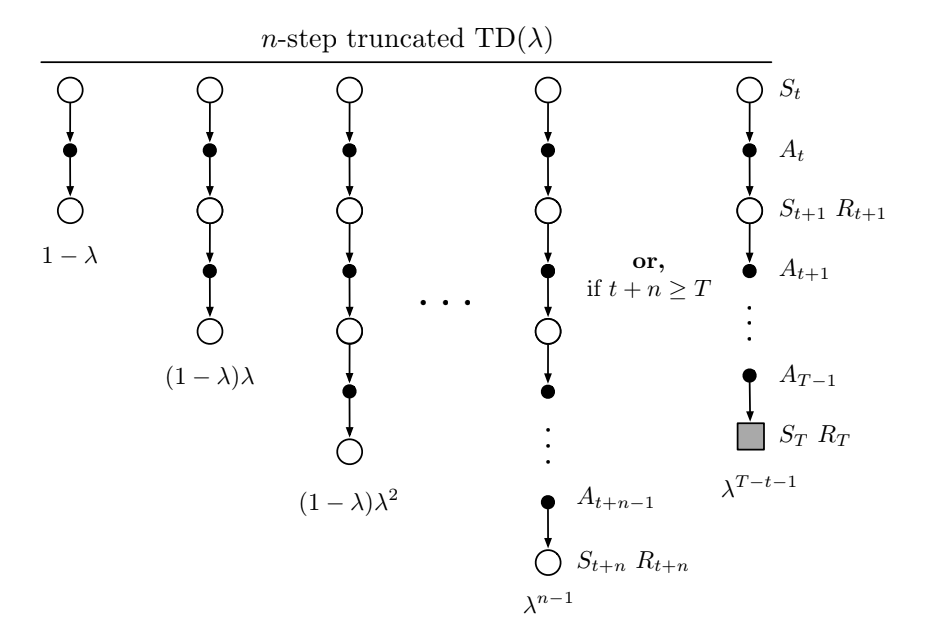
\includegraphics[width=0.5\textwidth]{truncated_td.png}
    \caption{Truncated TD}
\end{figure}
In $n$-step methods, updates are delayed $n$ steps and only considers the first $n$ rewards; in contrast, now we consider all $k$ ($1 < k < n$) returns in between.

\newpage
\subsection{Redoing updates: The online lambda-return algorithm}

\begin{itemize}
\item Truncation parameter involves a tradeoff: n should be later to be closer to the true $\lambda$-return, but it should also be sooner to influence behaviour earlier 
\item This is about getting both (at the cost of computational complexity) 
\end{itemize}

 At each time step we go back in time and redo all updates since the beginning of the episode 
\begin{itemize}
\item the new updates are better because they take the time step’s new data 
\end{itemize}

 Convention: 
\begin{itemize}
\item $\mathbf{w}_0^h$ is the first weight vector in each sequence that is inherited from the previous sequence 
\item the last weight vector in each sequence $\mathbf{w}_h^h$ defines the ultimate weight-vector sequence of the algorithm 
\item Example of the first 3 sequences: 
\end{itemize}
\begin{align*}
h = 1: \quad \quad & \mathbf{w}_1^1 \doteq \mathbf{w}_0^1 + \alpha [G_{0:1}^{\lambda} - \hat{v}(S_0, \mathbf{w}_0^1)] \nabla \hat{v}(S_0, \mathbf{w}_0^1)
\end{align*} 
\begin{align*}
h = 2: \quad \quad & \mathbf{w}_1^2 \doteq \mathbf{w}_0^2 + \alpha [G_{0:2}^{\lambda} - \hat{v}(S_0, \mathbf{w}_0^2)] \nabla \hat{v}(S_0, \mathbf{w}_0^2)\\
 & \mathbf{w}_2^2 \doteq \mathbf{w}_1^2 + \alpha [G_{1:2}^{\lambda} - \hat{v}(S_1, \mathbf{w}_1^2)] \nabla \hat{v}(S_1, \mathbf{w}_1^2)
\end{align*} 
\begin{align*}
h = 3: \quad \quad & \mathbf{w}_1^3 \doteq \mathbf{w}_0^3 + \alpha [G_{0:3}^{\lambda} - \hat{v}(S_0, \mathbf{w}_0^3)] \nabla \hat{v}(S_0, \mathbf{w}_0^3)\\
 & \mathbf{w}_2^3 \doteq \mathbf{w}_1^3 + \alpha [G_{1:3}^{\lambda} - \hat{v}(S_1, \mathbf{w}_1^3)] \nabla \hat{v}(S_1, \mathbf{w}_1^3)\\
 & \mathbf{w}_3^3 \doteq \mathbf{w}_2^3 + \alpha [G_{2:3}^{\lambda} - \hat{v}(S_2, \mathbf{w}_2^3)] \nabla \hat{v}(S_2, \mathbf{w}_2^3)
\end{align*} 

 General form of the update:
\begin{align}\mathbf{w}_{t+1}^h = \mathbf{w}_t^h + \alpha [G_{t:h}^{\lambda} - \hat{v}(S_t, \mathbf{w}_t^h)] \nabla \hat{v}(S_t, \mathbf{w}_t^h) \label{eq:12.9}\tag{12.9}\end{align}

 This update, along $\mathbf{w}_t = \mathbf{w}_t^t$ defines the \textbf{online $\lambda$-return algorithm} 

\subsection{True online TD-lambda}

\begin{itemize}
\item the algorithm from 12.4 is an ideal that online TD($\lambda$) will try to approximate 
\item we use ET to invert the forward view to a backward view 
\item “true” because it’s “truer” to the ideal online $\lambda$-return algorithm than the TD($\lambda$) actually is 
\end{itemize}
 The sequence of weight vectors produced by the online $\lambda$-return algorithm can be arranged in a triangle: 
\begin{figure}[h!]
    \centering
     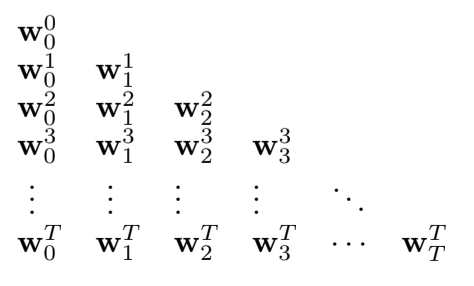
\includegraphics[width=0.8\textwidth]{triangle.png}
\end{figure}
\begin{itemize}
\item one row is produced at each time step 
\item turns out that only the weight vectors in the diagonal are really needed 
\item first one $\mathbf{w}_0^0$ is the input, last one $\mathbf{w}_T^T$ is the final weight vector, and the intermediate values are used to bootstrap the n-step returns of the updates 
\item if we can find a way to compute each last vector from the last vector of the previous row, we’re good! 
\end{itemize}
\begin{align}\mathbf{w}_{t+1} = \mathbf{w}_t + \alpha \delta_t \mathbf{z}_t + \alpha (\mathbf{w}_t^{\top} \mathbf{x}_t - \mathbf{w}_{t-1}^{\top} \mathbf{x}_t) (\mathbf{z}_t - \mathbf{x}_t) \label{eq:12.10}\tag{12.10}\end{align}
\begin{itemize}
\item shorthand $\mathbf{x}_t = \mathbf{x}(S_t)$ 
\item $\delta_t$ is defined as in TD($\lambda$) 
\item $\mathbf{z}_t$ is the \textbf{dutch trace} defined by: 
\end{itemize}
\begin{align}\mathbf{z}_t = \gamma \lambda \mathbf{z}_{t-1} + (1 - \alpha \gamma \lambda \mathbf{z}_{t-1}^{\top} \mathbf{x}_t) \mathbf{x}_t \label{eq:12.11}\tag{12.11}\end{align}

\begin{itemize}
\item proved to produce the same sequence of weights than online $\lambda$-return algorithm 
\item memory requirements same as TD($\lambda$) 
\item 50\% more computation because there is one more inner-product in the ET update 
\end{itemize}
\begin{figure}[h!]
    \centering
     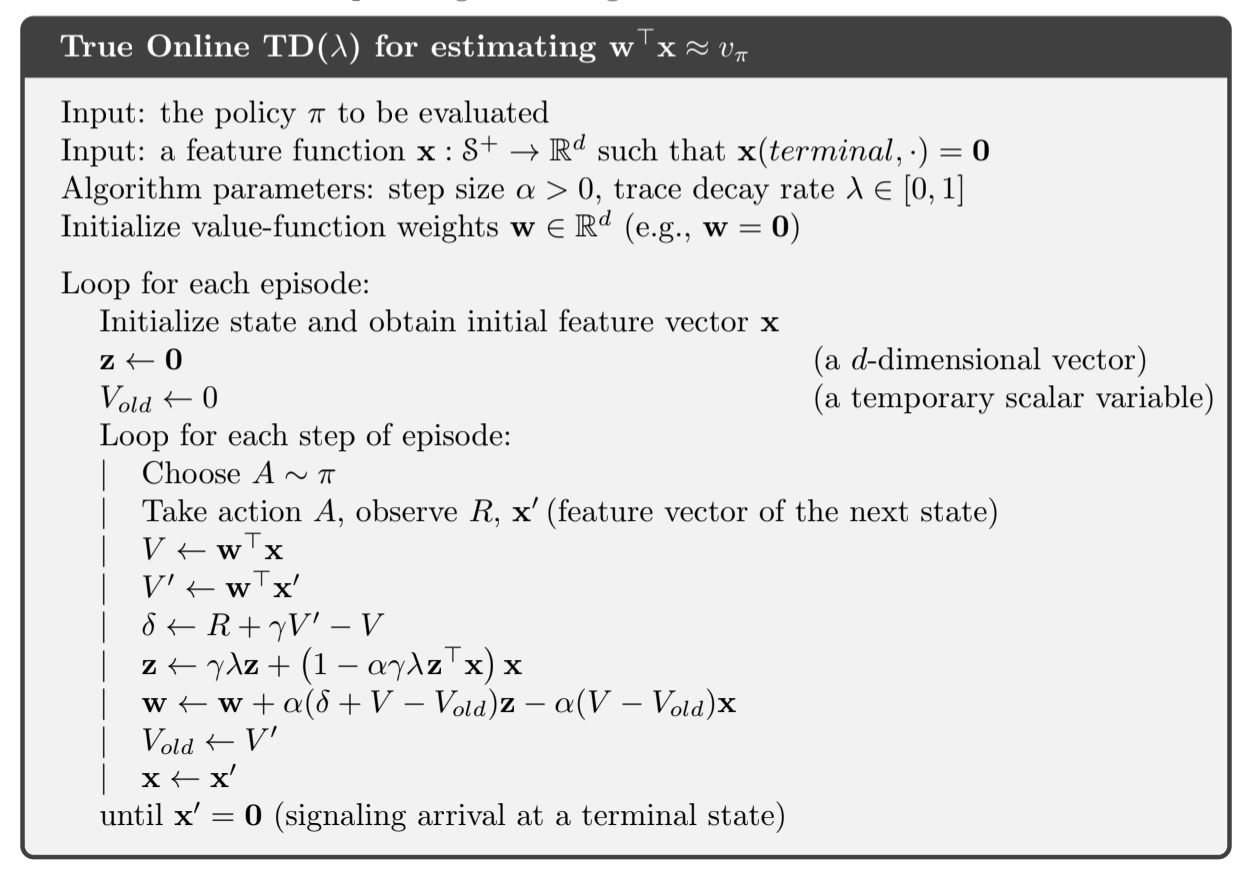
\includegraphics[width=0.8\textwidth]{true_online_td.png}
    \caption{ True online TD }
\end{figure}

\paragraph{summary}
\begin{itemize}
\item accumulating trace (TD($\lambda$)): $\mathbf{z}_t = \gamma \lambda \mathbf{z}_{t-1} + \nabla \hat{v}(S_t, \mathbf{w}_t) \quad 0 \leq t \leq T$
\begin{itemize}
	\item can be used for nonlinear FA
\end{itemize}
\item dutch trace (True online TD($\lambda$)): $\mathbf{z}_t = \gamma \lambda \mathbf{z}_{t-1} + (1 - \alpha \gamma \lambda \mathbf{z}_{t-1}^{\top} \mathbf{x}_t) \mathbf{x}_t$
\begin{itemize}
	\item same memory requirement as accumulating trace
	\item per-step computation increased about 50\%
	\item NOT for nonlinear FA
\end{itemize}
\item replacing trace: $z_{i,t} = 1$ if $x_{i,t} = 1$, else $\gamma\lambda z_{i,t-1}$
\begin{itemize}
	\item only for tabular case, or for binary feature vectors
	\item crude approx. to dutch trace
\end{itemize}
\end{itemize}

\subsection{Dutch Traces in Monte Carlo Learning}

\begin{itemize}
\item ET has nothing to do with TD, though they are closely associated
\item ET is not specific to TD, it can also be used in MC
\item The need for ET arise whenever one tries to learn long-term predictions in an efficient manner
\end{itemize}

\subsection{Sarsa($\lambda$)}

\begin{itemize}
\item extend eligibility traces to learn action-values 
\item to learn approximate values we need to use the action-value form of the n-step return: 
\end{itemize}
\begin{align}
G_{t:t+n} = R_{t+1} + ... + \gamma^{n-1} R_{t+n} + \gamma^n \hat{q}(S_{t+n}, A_{t+n}, \mathbf{w}_{t+n-1}) \quad \quad t + n < T \label{eq:12.12}\tag{12.12}
\end{align}
\begin{itemize}
\item We use this return to form the action-value form of the truncated $\lambda$-return 
\item $G_t^{\lambda} \doteq G_{t:\infty}^{\lambda}$ 
\item The action-value form of the $\lambda$-return algorithm uses $\hat{q}$ rather than $\hat{v}$: 
\end{itemize}
\begin{align}
\mathbf{w}_{t+1} = \mathbf{w}_{t} + \alpha [G_t^\lambda - \hat{q}(S_t, A_t, \mathbf{w}_{t})] \nabla \hat{q}(S_t, A_t, \mathbf{w}_{t}) \label{eq:12.13}\tag{12.13}
\end{align}
\begin{itemize}
\item This is the forward view. The backup diagram is similar to the TD($\lambda$): 
\end{itemize}
\begin{figure}[h!]
    \centering
     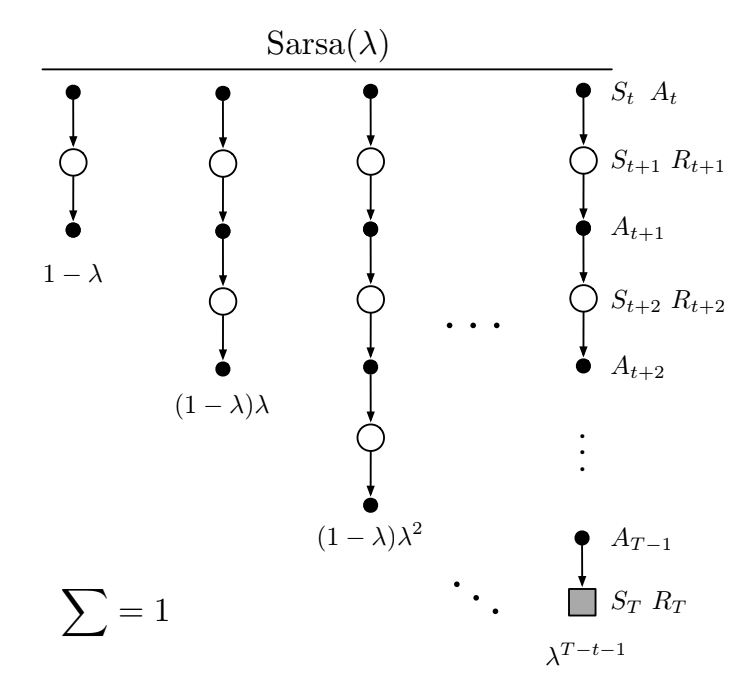
\includegraphics[width=0.3\textwidth]{sarsa_lambda_backup.png}
    \caption{ Sarsa lambda backup }
\end{figure}
\newpage
\begin{itemize}
\item first update: one step, second update: 2 steps, final update: complete return 
\item the weighting on each n-step return is the same as TD($\lambda$) 
\end{itemize}
 The backward view of the temporal difference method for action-values, Sarsa($\lambda$), is defined by: 
\begin{align}
\mathbf{w}_{t+1} = \mathbf{w}_{t} + \alpha \delta_t \mathbf{z}_{t}  \label{eq:12.14}\tag{12.14}
\end{align}
 Where the TD error is the action-values one: 
\begin{align}
\delta_t = R_{t+1} + \gamma \hat{q}(S_{t+1}, A_{t+1}, \mathbf{w}_{t}) - \hat{q}(S_{t}, A_{t}, \mathbf{w}_{t})  \label{eq:12.15}\tag{12.15}
\end{align}
 Action-value form of the eligibility trace (init to 0): 
\begin{align}
\mathbf{z}_{t} = \gamma \lambda \mathbf{z}_{t-1} + \nabla \hat{q}(S_t, A_t, \mathbf{w}_{t})  \label{eq:12.16}\tag{12.16}
\end{align}
 Pseudocode (using binary features): 
\begin{figure}[h!]
    \centering
     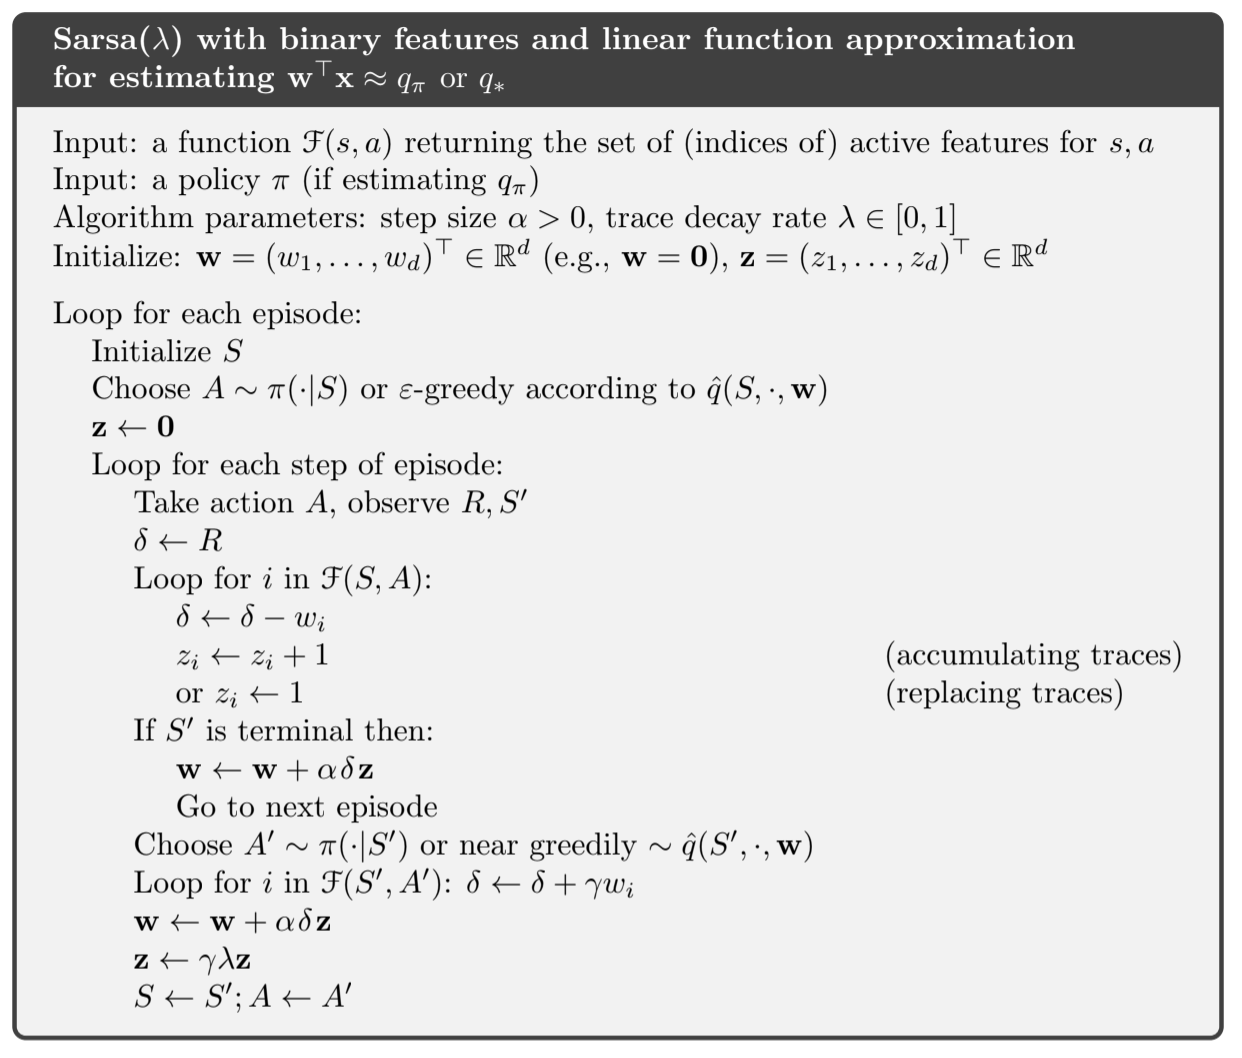
\includegraphics[width=0.8\textwidth]{sarsa_lambda_binary.png}
    \caption{ Sarsa lambda with binary features }
\end{figure}

 Illustrative example of different methods: 
\begin{figure}[h!]
    \centering
     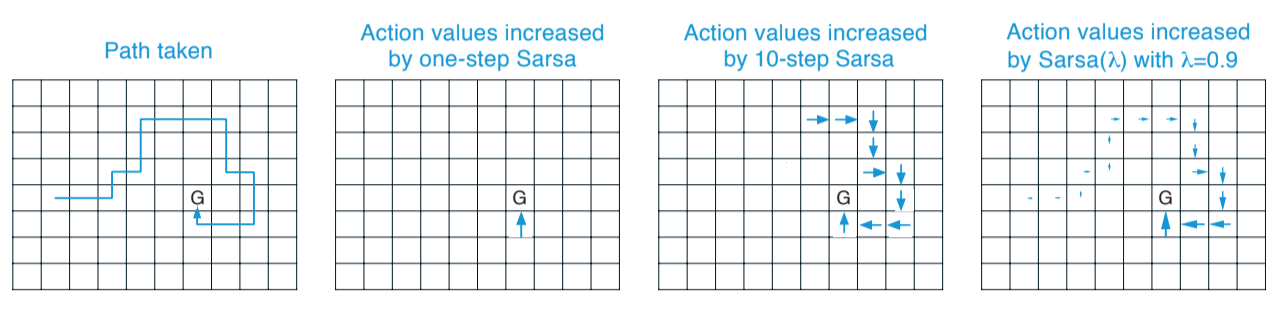
\includegraphics[width=0.8\textwidth]{sarsas.png}
    \caption{ Updates made for different methods in a gridworld example. A one-step method would update only the last value, a n-step would update n values, and the use of eligibility traces spread the update using a fading strategy }
\end{figure}

 The Linear function approximation case has an exact $O(d)$ implementation called \textbf{True Online Sarsa($\lambda$)}. 


\subsection{Variable $\lambda$ and $\gamma$}

\begin{itemize}
\item To generalize our TD learning algorithms, we need to generalize the degree of bootstrapping and discounting beyond constant parameters $\lambda$ and $\gamma$ 
\item Now the parameter have a varying value at each time step, $\lambda_t = \lambda(S_t, A_t)$ and $\gamma_t = \gamma(S_t)$ 
\end{itemize}

\paragraph{gamma}
 The function $\gamma$ is a \textbf{termination function} and it now changes the return (the fundamntal Random Variable (RV) whose expectation we seek to estimate) 
\begin{align*}
G_t & = R_{t+1} + \gamma_{t+1} G_{t+1}\\
 & = R_{t+1} + \gamma_{t+1} R_{t+2} + \gamma_{t+1} \gamma_{t+2} R_{t+3} + ...\\
 & = \sum_{k=t}^{\infty} R_{k+1} \prod_{i=t+1}^k \gamma_i \label{eq:12.17}\tag{12.17}
\end{align*} 
\begin{itemize}
\item to ensure the sums are finite, we require that $\prod_{k=t}^{\infty} \gamma_k = 0$ with probability $1$ for all $t$. 
\item this definition allows to get rid of episodes, a terminal state just becomes a state with $\gamma = 0$ and which transitions to a start state 
\end{itemize}

\paragraph{lambda}
 Generalization to variable bootstrapping gives a new state-based $\lambda$-return: 
\begin{align}
G_t^{\lambda s} = R_{t+1} + \gamma_{t+1} \big( (1 - \lambda_{t+1}) \hat{v}(S_{t+1}, \mathbf{w}_{t}) + \lambda_{t+1} G_{t+1}^{\lambda s}\big) \label{eq:12.18}\tag{12.18}
\end{align}

 First reward + possibly a second term according to $\gamma_{t+1}$, and that term is 
\begin{itemize}
\item the estimated value at the state if we’re bootstrapping 
\item the $\lambda$-return for the next timestep if we are not 
\end{itemize}
 Notation: 
\begin{itemize}
\item s superscript: bootstraps from state-values 
\item a superscript: bootstraps from action-values 
\end{itemize}
 Action-based lambda-return in Sarsa form: 
\begin{align}
G_t^{\lambda a} = R_{t+1} + \gamma_{t+1} \big( (1 - \lambda_{t+1}) \hat{q}(S_{t+1}, A_{t+1}, \mathbf{w}_{t}) + \lambda_{t+1} G_{t+1}^{\lambda a}\big) \label{eq:12.19}\tag{12.19}
\end{align}
 Expected Sarsa form: 
\begin{align}
G_t^{\lambda a} = R_{t+1} + \gamma_{t+1} \big( (1 - \lambda_{t+1}) \bar{V}_t(S_{t+1}) + \lambda_{t+1} G_{t+1}^{\lambda a}\big) \label{eq:12.20}\tag{12.20}
\end{align}
 where $V$ is generalized to function approximation: 
\begin{align}
\bar{V}(s) = \sum_a \pi(a|s) \hat{q}(s, a, \mathbf{w}_{t}) \label{eq:12.21}\tag{12.21}
\end{align}

\subsection{Off-policy Eligibility Traces with Control Variates}

 \textbf{Goal} 
\begin{itemize}
\item We want to incorporate importance sampling with eligibility traces to be able to use off-policy algorithms. To do that, we need:
    \begin{itemize}
    \item To formulate the return 
    \item Use the return in the formulation of the target for the $\mathbf{w}$ update 
    \item Get the eligibility trace $\mathbf{z}$ update 
    \end{itemize}
\end{itemize}

 \textbf{Context} 
\begin{itemize}
\item As a reminder, importance sampling $\rho_t = \frac{\pi(A_t|S_t)}{b(A_t|S_t)}$ is a quantity that is used to weight the return obtained using the behaviour policy, to be able to learn off-policy 
\item It often leads to solution that have a high variance, and are slow to converge 
\item \textbf{Control variates} aims to reduce the variance of the initial estimator (which includes $\rho$), by subtracting a baseline that has $0$ expectation. 
\item \textbf{Per decision} importance sampling with control variates was introduced in chap 7.4, and here we develop the bootstrapping version of it: 
\end{itemize}

 \textbf{1: Express return with control variates}
\begin{align}
G_t^{\lambda s} = \rho_t \Big( R_{t+1} + \gamma_{t+1} \big( (1 - \lambda_{t+1}) \hat{v}(S_{t+1}, \mathbf{w}_{t}) + \lambda_{t+1} G_{t+1}^{\lambda s}\big) \Big) + (1 - \rho_t) \hat{v}(S_{t}, \mathbf{w}_{t}) \label{eq:12.22}\tag{12.22}
\end{align} 

 In this formulation of the return, the control variate is the $(1 - \rho_t) \hat{v}(S_{t}, \mathbf{w}_{t})$ part, which prevents the return to be $0$ if the experienced trajectory has no chance of occurring under the target policy for example. 

 \textbf{2: Approximation of the truncated return} 
To use this return in a practical algorithm, we will use the \textbf{truncated} version of the return, which can be approximated as the sum of state-based TD errors $\delta_t^s$: 

\begin{align}
\delta_t^s = R_{t+1} + \gamma_{t+1} \hat{v}(S_{t+1}, \mathbf{w}_{t}) - \hat{v}(S_{t}, \mathbf{w}_{t}) \label{eq:12.23}\tag{12.23}
\end{align}

\begin{align}
G_t^{\lambda s} \approx \hat{v}(S_{t}, \mathbf{w}_{t}) + \rho_t \sum_{k=t}^{\infty} \delta_k^s \prod_{i=t+1}^k \gamma_i \lambda_i \rho_i \label{eq:12.24}\tag{12.24}
\end{align}

 \textbf{3: Write the forward view update}
We can use the truncated return in the forward view update (i.e. without eligibility traces): 

 
\begin{align}
\mathbf{w}_{t+1} & = \mathbf{w}_{t} + \alpha [G_t^{\lambda s} - \hat{v}(S_t, \mathbf{w}_{t})] \nabla \hat{v}(S_t, \mathbf{w}_{t}) \label{eq:12.25}\tag{12.25}\\
 & \approx \mathbf{w}_{t} + \alpha \rho_t \Big( \sum_{k=t}^{\infty} \delta_k^s \prod_{i=t+1}^k \gamma_i \lambda_i \rho_i\Big) \nabla \hat{v}(S_t, \mathbf{w}_{t}) \label{eq:12.26}\tag{12.26}
\end{align} 

 \textbf{4: Eligibility trace update} 
This update kinda looks like an eligibility-based TD update: the product product would be the ET and it is multiplied by the TD error. But the relationship we’re looking for is an (approximate) equivalence between the forward view update, summed over time, and the backward view update, also summed over time. Let’s start with the forward view update that we sum over time: 
\begin{align}
\sum_{t=0}^{\infty} (\mathbf{w}_{t+1} - \mathbf{w}_{t}) & \approx \sum_{t=1}^{\infty} \sum_{k=t}^{\infty} \alpha \rho_t \delta_k^s \nabla \hat{v}(S_t, \mathbf{w}_t) \prod_{i=t+1}^k \gamma_i \lambda_i \rho_i \label{eq:12.27}\tag{12.27}\\
& = \sum_{k=1}^{\infty} \sum_{t=1}^{k} \alpha \rho_t \nabla \hat{v}(S_t, \mathbf{w}_t) \delta_k^s \prod_{i=t+1}^k \gamma_i \lambda_i \rho_i \label{eq:12.28}\tag{12.28}\\
& = \sum_{k=1}^{\infty} \alpha \delta_k^s \sum_{t=1}^{k} \rho_t \nabla \hat{v}(S_t, \mathbf{w}_t) \prod_{i=t+1}^k \gamma_i \lambda_i \rho_i \label{eq:12.29}\tag{12.29}\\
\end{align} 

\begin{itemize}
\item \ref{eq:12.28} uses the summation rule $\sum_{t=x}^y \sum_{k=t}^y = \sum_{k=x}^y \sum_{t=x}^k$ 
\end{itemize}

 If the entire expression from the second sum left could be written and updated incrementally as an ET, we would have the sum of the backward-view TD update. This is derived in details in the book, but in the end we get the general accumilating trace for state values: 
\begin{align}
\mathbf{z}_{t} = \rho_t (\gamma_t \lambda_t \mathbf{z}_{t-1} + \nabla \hat{v}(S_t, \mathbf{w}_{t})) \label{eq:12.30}\tag{12.30}
\end{align}

 \textbf{5: Combine everything to get the semi-gradient update} 
This ET can be combined with the usual semi-gradient parameter update rule for TD($\lambda$) \ref{eq:12.6} to form a general TD($\lambda$) algorithm: 
\begin{itemize}
\item on-policy $\rho_t$ is always one and we get the usual accumulating trace 
\item we now have the off-polcy version 
\end{itemize}

 -> Extension to the action-values is simplest with Expected Sarsa 

 At $\lambda = 0$ these algorithms are related to MC, but in a more subtle way since we don’t have any episodes.
-> For exact equivalence see PTD($\lambda$) and PQ($\lambda$) [P = provisional] 

\subsection{Watkins’s Q($\lambda$) to Tree-Backup($\lambda$)}

\begin{itemize}
\item Extend Q-learning to eligibility traces has been the subject of many methods, Watkins’s is the first one 
\item Basic principle: decay the ET the usual way as long as a greedy action is taken 
\item Cut the traces to $0$ when a non-greedy action is taken 
\end{itemize}

 Backup diagram: 

\begin{figure}[h!]
    \centering
     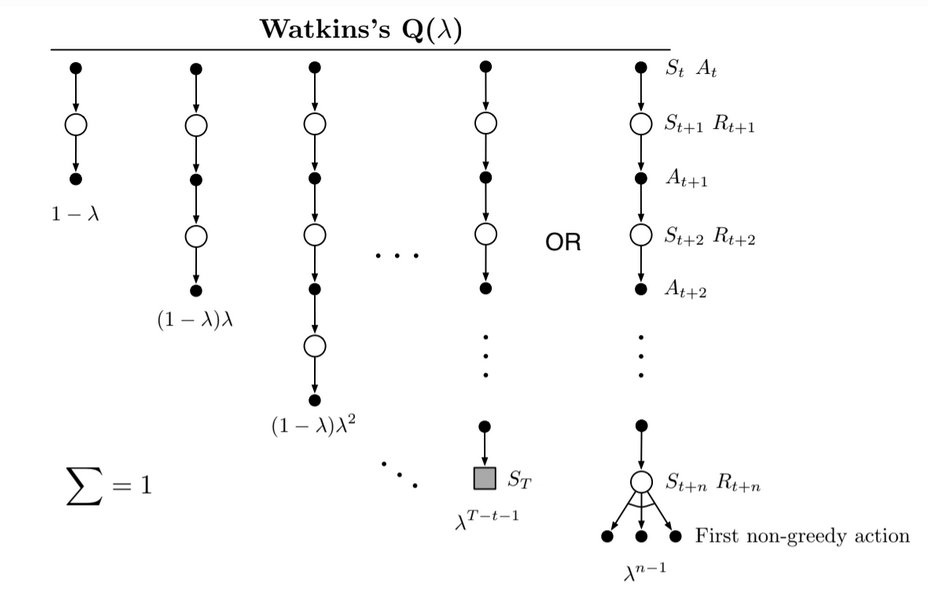
\includegraphics[width=0.8\textwidth]{watkins.png}
    \caption{ Watkins's Q($\lambda$) backup diagram. The series of update ends with the first non-greedy action (or with the end of the episode) }
\end{figure}


\paragraph{ET with Tree Backups (TB($\lambda$))}
\begin{itemize}
\item ‘true’ succesor to Q-learning because it has no importance sampling 
\end{itemize}

 Backup diagram: 

\begin{figure}[h!]
    \centering
     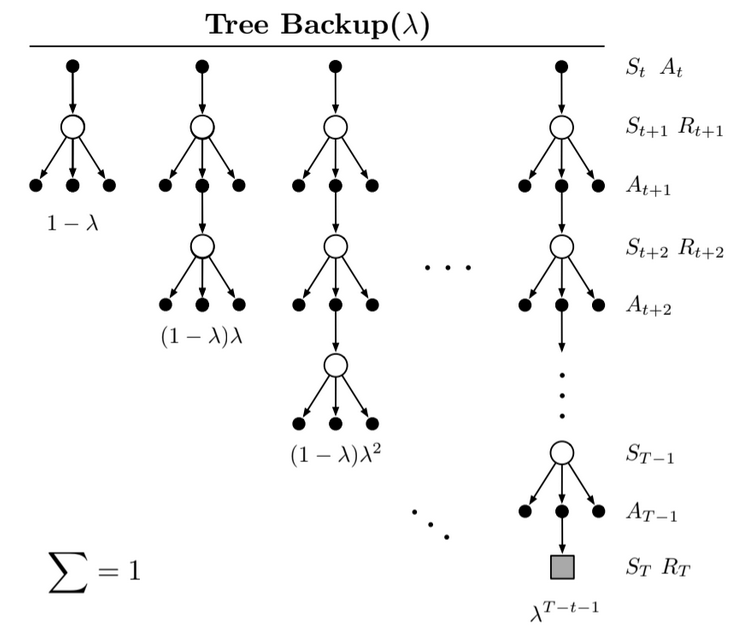
\includegraphics[width=0.8\textwidth]{tb_lambda.png}
    \caption{ Backup diagram for the TB($\lambda$) algorithm }
\end{figure}


 The tree-backup updates are weighted the usual way depending on bootstrapping parameter $\lambda$
For the return we start with the recursive form of the $\lambda$-return using action values, and then expand the bootstrapping case of the target: 
\begin{align*}
\hspace*{-10cm}G_t^{\lambda a} & \doteq R_{t+1} + \gamma_{t+1} \Big( (1 - \lambda_{t+1}) \bar{V}_t(S_{t+1}) \\
& + \lambda_{t+1} \big[ \sum_{a \neq A_{t+1}} \pi(a|S_{t+1}) \hat{q}(S_{t+1}, a, \mathbf{w}_t) + \pi(A_{t+1}| S_{t+1}) G_{t+1}^{\lambda a} \big] \Big)\\\label{eq:12.31}\tag{12.31}\\
& = R_{t+1} + \gamma_{t+1} \label{eq:12.32}\tag{12.32}
\end{align*} 
 Can be written approximately as a sum of TD errors: 
\begin{align}
G_t^{\lambda a} \approx \hat{q}(S_{t}, A_t, \mathbf{w}_{t}) + \rho_t \sum_{k=t}^{\infty} \delta_k^a \prod_{i=t+1}^k \gamma_i \lambda_i \pi(A_i|S_i) \label{eq:12.33}\tag{12.33}
\end{align}

 Using expectation form of the action-based TD error.
Trace update involving target-policy probabilities of the selected actions: 

\begin{align}
\mathbf{z}_{t+1} = \gamma_t \lambda_t \pi(A_t| S_t) \mathbf{z}_{t-1} + \nabla \hat{q}(S_t, A_t, \mathbf{w}_{t}) \label{eq:12.34}\tag{12.34}
\end{align}

 We can combine this to the usual parameter update rule \ref{eq:12.6} to get the TB($\lambda$) algorithm: 
\begin{align}\mathbf{w}_{t+1} = \mathbf{w}_t + \alpha \delta_t \mathbf{z}_t\end{align}

\subsection{Stable off-policy methods with traces}

 Here we present 4 of the most important ways. All are based on either Gradient-TD or Emphatic-TD and assume linear function approximation. 

\paragraph{GTD($\lambda$)}
\begin{itemize}
\item analogous to TDC 
\item our goal is to learn a parameter $\mathbf{w}_{t}$ such that $\hat{v}(s, \mathbf{w}) = \mathbf{w}_t^{\top} \mathbf{x}(s) \approx v_{\pi}(s)$ even from data due to the behaviour policy $b$ 
\end{itemize}
\begin{align}
\mathbf{w}_{t+1} = \mathbf{w}_t + \alpha \delta_t^s \mathbf{z}_t - \alpha \gamma_{t+1}(1 - \lambda_{t+1})(\mathbf{z}_t^{\top} \mathbf{v}_t) \mathbf{x}_{t+1} \label{eq:12.35}\tag{12.35}
\end{align}
 with: 
\begin{align}
\mathbf{v}_{t+1} = \mathbf{v}_t + \beta \delta_t^s \mathbf{z}_t - \beta (\mathbf{v}_t^{\top} \mathbf{x}_t) \mathbf{x}_t \label{eq:12.36}\tag{12.36}
\end{align}

\begin{itemize}
\item $\mathbf{v}$ is a vector (defined in 11.7) the same size as $\mathbf{w}$ 
\item $\beta$ is a second step-size parameter 
\end{itemize}

\paragraph{GQ($\lambda$)}
\begin{itemize}
\item Gradient-TD algo for action-values with ET 
\item Goal: learn $\mathbf{w}_t$ such that $\hat{q}(s, a, \mathbf{w}_t) = \mathbf{w}_t^{\top} \mathbf{x}(s, a) \approx q_{\pi}(s, a)$ from off-policy data 
\end{itemize}
\begin{align}
\mathbf{w}_{t+1} = \mathbf{w}_t + \alpha \delta_t^a \mathbf{z}_t - \alpha \gamma_{t+1} (1 - \lambda_{t+1}) (\mathbf{z}_t^{\top} \mathbf{v}_t) \bar{\mathbf{x}}_{t+1} \label{eq:12.37}\tag{12.37}
\end{align}
 where $\bar{\mathbf{x}}_{t}$ is the average feature vector for $S_t$ under target policy: 
\begin{align}
\bar{\mathbf{x}}_{t} = \sum_a \pi(a|S_t) \mathbf{x}(S_t, a) \label{eq:12.38}\tag{12.38}
\end{align}

 $\delta_t^a$ is the expectation form TD error: 
\begin{align}
\delta_t^a = R_{t+1} + \gamma_{t+1} \mathbf{w}_t^{\top} \bar{\mathbf{x}}_{t+1} -  \mathbf{w}_t^{\top} \mathbf{x}_{t} \label{eq:12.39}\tag{12.39}
\end{align}

 The rest is the same as GTD including the update for $v$. 

\paragraph{HTD($\lambda$)}
\begin{itemize}
\item Hybrid state-value algorithm combining GTD($\lambda$) and TD($\lambda$) 
\item It is a strict generalization of TD($\lambda$) to off-policy, meaning that we find TD($\lambda$) if $\rho_t = 1$ 
\end{itemize}

 
\begin{align}
\mathbf{w}_{t+1} & \doteq \mathbf{w}_t + \alpha \delta_t^s \mathbf{z}_t + \alpha \big( (\mathbf{z}_t - \mathbf{z}_t^b)^{\top} \mathbf{v}_t \big) (\mathbf{x}_t - \gamma_{t+1} \mathbf{x}_{t+1}) \label{eq:12.40}\tag{12.40}\\
\mathbf{v}_{t+1} & \doteq \mathbf{v}_t + \beta \delta_t^s \mathbf{z}_t + \beta \big( {\mathbf{z}_t^b}^{\top} \mathbf{v}_t \big) (\mathbf{x}_t - \gamma_{t+1} \mathbf{x}_{t+1}), \quad \quad \text{with} \quad \mathbf{v}_{0} \doteq 0 \label{eq:12.41}\tag{12.41}\\
\mathbf{z}_{t} & \doteq \rho_t(\gamma_t \lambda_t \mathbf{z}_{t-1} + \mathbf{x}_t), \quad \quad \text{with} \quad \mathbf{z}_{-1} \doteq 0 \label{eq:12.42}\tag{12.42}\\
\mathbf{z}_{t}^b & \doteq \gamma_t \lambda_t \mathbf{z}_{t-1}^b + \mathbf{x}_t, \quad \quad \text{with} \quad \mathbf{z}_{-1}^b \doteq 0 \label{eq:12.43}\tag{12.43}
\end{align} 

 We have: 
\begin{itemize}
\item a second set of weights $\mathbf{v}$ 
\item a second set of eligibility traces $\mathbf{z}_t^b$ for the behaviour policy 
\item these $\mathbf{z}_t^b$ reduce to $\mathbf{z}_t$ if $\rho_t$ is 1, causing the last term to be $0$ and algorithm turning TD($\lambda$) 
\end{itemize}

\paragraph{Emphatic TD($\lambda$)}
\begin{itemize}
\item Extension of Emphatic-TD to eligibility traces 
\item high variance and potentially slow convergence 
\item good convergence guarantees and bootstrapping 
\end{itemize}

 
\begin{align}
\mathbf{w}_{t+1} & \doteq \mathbf{w}_t + \alpha \delta_t \mathbf{z}_t \label{eq:12.44}\tag{12.44}\\
\delta_{t} & \doteq R_{t+1} + \gamma_{t+1} \mathbf{w}_t^{\top} \mathbf{x}_{t+1} -  \mathbf{w}_t^{\top} \mathbf{x}_{t}\label{eq:12.45}\tag{12.45}\\
\mathbf{z}_{t} & \doteq \rho_t(\gamma_t \lambda_t \mathbf{z}_{t-1} + M_t \mathbf{x}_t) \label{eq:12.46}\tag{12.46}\\
M_{t} & \doteq \lambda_t I_t + (1 - \lambda_t) F_t \label{eq:12.47}\tag{12.47}\\
F_{t} & \doteq \rho_{t-1} \gamma_t F_{t-1} + I_t \label{eq:12.48}\tag{12.48}
\end{align} 

 With: 
\begin{itemize}
\item $M_t$ emphasis 
\item $F_t$ followon trace 
\item $I_t$ interest (chap 11.8)   
\item More details in Sutton 2015b 
\item Details on convergence properties: Yu’s counterexample to see difference with TD($\lambda$) (Ghiassian, Rafiee, and Sutton, 2016). 
\end{itemize}

\subsection{Conclusion}

\begin{itemize}
\item ET with TD errors provide an efficient, incremental way of shiftwing between TD and MC methods 
\item ET are more general than n-step methods 
\item MC may have advantages in non-Markov because they do not bootstrap, use ET on TD methods makes them closer to MC and thus more suited to non-Markov cases 
\item Beware: most of the times we are in a “deadly triad” scenario and we don’t have any convergence guarantee! 
\end{itemize}

\end{document}